\documentclass[t]{beamer}

% --- Theme and Color Setup ---
\usetheme{Madrid}

% Define the custom Orange color
\definecolor{BogaziciBlue}{RGB}{29, 79, 144} 

% Apply the orange color to the structure
\usecolortheme[named=BogaziciBlue]{structure}

% Fix footer colors to match the orange theme
\setbeamercolor{palette primary}{bg=BogaziciBlue,fg=white}
\setbeamercolor{palette secondary}{bg=BogaziciBlue!80!black,fg=white}
\setbeamercolor{palette tertiary}{bg=BogaziciBlue!60!black,fg=white}
\setbeamerfont{caption}{size=\footnotesize}

% Packages
\usepackage[utf8]{inputenc}
\usepackage{hyperref}
\usepackage{tikz} 
\usepackage{booktabs}
\usepackage{natbib}
\usepackage{graphicx}
\usepackage{amsmath}
\usepackage{amssymb}

% --- 1. CONFIGURATION FOR CONTENT SLIDES (Middle Pages) ---
\addtobeamertemplate{frametitle}{}{%
    \begin{tikzpicture}[remember picture,overlay]
        \node[anchor=north east, xshift=-0.3cm, yshift=0cm, inner sep=0pt] at (current page.north east) {
            
\includegraphics[height=1cm, keepaspectratio]{boun_white.png}
        };
    \end{tikzpicture}%
}

% --- 2. CONFIGURATION FOR FIRST & LAST PAGE ---
\newcommand{\FirstLastPageLayout}{
    \begin{tikzpicture}[remember picture,overlay]
        \node[anchor=north east, xshift=-0.3cm, yshift=0cm, inner sep=0pt] at (current page.north east) {
            
\includegraphics[height=1cm, keepaspectratio]{boun.png}
        };
        \node[anchor=south west, xshift=0.5cm, yshift=0.5cm] at (current page.south west) {
            \textcolor{BogaziciBlue}{\footnotesize Boğaziçi University}
        };
    \end{tikzpicture}
}

% --- Info ---
\title[Multi-Piano]{Multi-Piano: LAN Multiplayer Terminal Piano}
\subtitle{CMPE487}
\author{Ömer Faruk Erzurumluoğlu \and Berkay Keskin}
\institute[]{Department of Computer Engineering}
\date{June 2026}

\begin{document}

% --- Slide 1: Title Page ---
\begin{frame}
    \FirstLastPageLayout
    \titlepage
\end{frame}

\begin{frame}{Sections}
\begin{enumerate}
    \item Project Overview
    \item System Architecture
    \item Networking
    \item Audio Pipeline
    \item User Interface
    \item Deployment \& Future Work
\end{enumerate}
\end{frame}

\begin{frame}{Project Overview}
\textbf{Multi-Piano} is a LAN-based collaborative piano application with a terminal user interface (TUI).

\vspace{0.4cm}
\begin{itemize}
    \item Multiple players on the same network discover, host, and join lobbies.
    \item Notes are transmitted in near real time and played back with \textbf{clock-synchronised} audio.
\end{itemize}

\vspace{0.3cm}
\textbf{Goal:} demonstrate a lightweight multiplayer prototype combining discovery, mixed protocols, NTP-style clock sync, scheduled playout, and a full TUI.
\end{frame}

\begin{frame}{System Architecture}
\begin{center}
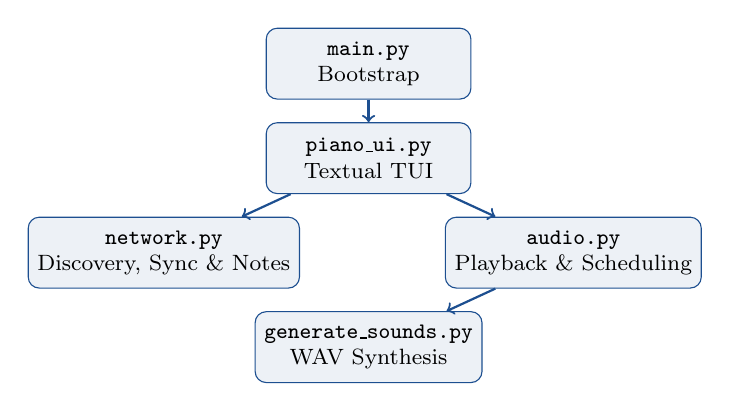
\begin{tikzpicture}[
    box/.style={draw=BogaziciBlue, fill=BogaziciBlue!8, rounded corners, minimum width=2.6cm, minimum height=0.9cm, align=center, font=\footnotesize},
    arr/.style={->, thick, BogaziciBlue}
]
    \node[box] (main) at (0,2.4) {\texttt{main.py}\\Bootstrap};
    \node[box] (ui) at (0,1.2) {\texttt{piano\_ui.py}\\Textual TUI};
    \node[box] (net) at (-2.6,0) {\texttt{network.py}\\Discovery, Sync \& Notes};
    \node[box] (audio) at (2.6,0) {\texttt{audio.py}\\Playback \& Scheduling};
    \node[box] (gen) at (0,-1.2) {\texttt{generate\_sounds.py}\\WAV Synthesis};

    \draw[arr] (main) -- (ui);
    \draw[arr] (ui) -- (net);
    \draw[arr] (ui) -- (audio);
    \draw[arr] (audio) -- (gen);
\end{tikzpicture}
\end{center}
\end{frame}

\begin{frame}{Networking — Three Channels}
We separate concerns into three network channels:

\vspace{0.3cm}
\begin{table}
\centering
\small
\begin{tabular}{clll}
\toprule
\textbf{Port} & \textbf{Protocol} & \textbf{Format} & \textbf{Role} \\
\midrule
12488 & UDP & JSON & Lobby discovery (broadcast) \\
12487 & TCP & length-prefixed JSON & Lobby management \\
12489 & UDP & binary + JSON & Note events \& clock sync \\
\bottomrule
\end{tabular}
\end{table}

\vspace{0.3cm}
\begin{itemize}
    \item \textbf{Discovery} finds open sessions without prior configuration.
    \item \textbf{TCP} maintains player membership and state synchronisation.
    \item \textbf{UDP 12489} carries 15-byte note packets and NTP-style \texttt{SYNC\_REQ}/\texttt{SYNC\_ACK} messages.
\end{itemize}
\end{frame}

\begin{frame}{Lobby Discovery (UDP 12488)}
\textbf{Client behaviour:}
\begin{itemize}
    \item Binds UDP port 12488.
    \item Sends \texttt{DISCOVER} broadcasts; listens for \texttt{LOBBY\_REPLY} responses.
\end{itemize}

\vspace{0.3cm}
\textbf{Host behaviour:}
\begin{itemize}
    \item Replies to discoverers with lobby name, host IP, TCP port, and active player count.
\end{itemize}

\end{frame}

\begin{frame}{Lobby Management (TCP 12487)}

\vspace{0.3cm}
\textbf{Join flow:}
\begin{enumerate}
    \item Client connects to \texttt{(host\_ip, 12487)}.
    \item Client sends \texttt{\{"type": "JOIN", "SENDER\_NAME": ..., "SENDER\_IP": ...\}}.
    \item Host accepts, stores the socket, and appends the client IP to \texttt{peer\_ips}.
    \item Host broadcasts \texttt{STATE\_UPDATE} with the current player list to all clients.
    \item Both sides start a clock-sync loop (every 5 s) over UDP 12489.
\end{enumerate}

\end{frame}

\begin{frame}{Clock Synchronisation}
\vspace{-0.5cm}  
\textbf{NTP-style exchange} (JSON on UDP 12489, every 5\,s):

\vspace{0.2cm}
\begin{center}
\small
\begin{tabular}{rcl}
    Peer A & & Peer B \\
    $t_1 = \texttt{time.time()}$ & & \\
    & $\xrightarrow{\texttt{SYNC\_REQ}\{t_1\}}$ & \\
    & & $t_2 = \texttt{time.time()}$ \\
    & & $t_3 = \texttt{time.time()}$ \\
    & $\xleftarrow{\texttt{SYNC\_ACK}\{t_1,t_2,t_3\}}$ & \\
    $t_4 = \texttt{time.time()}$ & & \\
\end{tabular}
\end{center}

\vspace{0.3cm}
\textbf{Offset calculation} (peer clock $-$ local clock):
\[
    \text{offset} = \frac{(t_2 - t_1) + (t_3 - t_4)}{2}
\]

\begin{itemize}
    \item Trip delays cancel; result is the pure clock difference.
    \item Both sides sync with each other; host syncs with every guest.
    \item Receiver converts a sender timestamp.
\end{itemize}
\end{frame}

\begin{frame}{Note Streaming \& Scheduled Playback}
\vspace{-0.5cm}
\textbf{Note packet} (15 bytes, little-endian, UDP 12489):

\vspace{0.1cm}
\small\texttt{seq (u32) $|$ play\_at (f64) $|$ note\_id (u8) $|$ action (u8) $|$ velocity (u8)}

\normalsize
\vspace{0.3cm}
\textbf{Sender} (on key press):
\begin{itemize}
    \item Computes \texttt{play\_at = time.time$()$ + 30\,ms} and fires a local \texttt{Timer} for own audio.
    \item Broadcasts the packet with \texttt{play\_at} embedded so every peer targets the same instant.
\end{itemize}

\vspace{0.3cm}
\textbf{Receiver — NoteScheduler}:
\begin{itemize}
    \item Converts: \texttt{local\_play\_at = play\_at $-$ offset}.
    \item Inserts into a \textbf{monotonic priority queue}.
    \item Background thread sleeps until \texttt{local\_play\_at}, then plays the note.
    \item Events more than 200\,ms overdue are discarded.
\end{itemize}
\end{frame}

% --- Final page ---
\begin{frame}[c]
    \FirstLastPageLayout
    \centering
    \Huge \textcolor{BogaziciBlue}{Thank you for your attention}

    \vspace{1.5cm}
    \normalsize
    \textbf{Ömer Faruk Erzurumluoğlu} \\
    \textbf{Muhammet Berkay Keskin} \\
    \vspace{0.3cm}
    \href{mailto:omer.erzurumluoglu@std.bogazici.edu.tr}{omer.erzurumluoglu@std.bogazici.edu.tr}\\
    \href{mailto:muhammet.keskin@std.bogazici.edu.tr}{muhammet.keskin@std.bogazici.edu.tr}
\end{frame}

\end{document}